%!TEX root = ../main.tex

\setcounter{chapter}{7}

\chapter{模型部署}
\label{ch:deploy}

在前面的章节中,我们讲述了机器学习模型训练系统的基本组成,这一章节我们将讲述模型部署的相关知识。模型部署是将训练好的模型部署到运行环境中进行推理的过程,模型部署的过程中需要解决训练模型到推理模型的转换,硬件资源对模型的限制,模型推理的时延、功耗、内存占用等指标对整个系统的影响以及模型的安全等一系列的问题。

本章将主要介绍机器学习模型部署的主要流程,包括训练模型到推理模型的转换、适应硬件限制的模型压缩技术、模型推理及性能优化以及模型的安全保护,最后我们会给出一个模型部署端到端的实践用例。

本章的学习目标包括:
\begin{itemize}
    \item 了解训练模型到推理模型转换及优化
    \item 掌握模型压缩的常用方法:量化、稀疏和知识蒸馏
    \item 掌握模型推理的流程及常用的性能优化的技术
    \item 了解模型安全保护的常用方法
\end{itemize}

\section{概述}



模型完成训练后,需要将模型及参数持久化成文件,不同的训练框架导出的模型文件中存储的数据结构不同,这给模型的推理系统带来了不便。推理系统为了支持不同的训练框架的模型,需要将模型文件中的数据转换成统一的数据结构。此外,在训练模型转换成推理模型的过程中,需要进行一些如算子融合、常量折叠等模型的优化以提升推理的性能。

推理模型部署到不同的场景,需要满足不同的硬件设备的限制,例如,在具有强大算力的计算中心或数据中心的服务器上可以部署大规模的模型,而在边缘侧服务器、个人电脑以及智能手机上算力和内存则相对有限,部署的模型的规模就相应地要降低。在超低功耗的微控制器上,则只能部署非常简单的机器学习模型。此外,不同硬件对于不同数据类型(如FP32、FP16、BF16、INT8等)的支持程度也不相同。为了满足这些硬件的限制,在有些场景下需要对训练好的模型进行压缩,降低模型的复杂度或者数据的精度,减少模型的参数,以适应硬件的限制。

模型部署到运行环境中执行推理,推理的时延、内存占用、功耗等是影响用户使用的关键因素,优化模型推理的方式有两种,一是设计专有的机器学习的芯片,相对于通用的计算芯片,这些专有芯片一般在能效比上具有很大的优势。二是通过软硬协同最大程度地发挥硬件的能力。对于第二种方式,以CPU为例,如何切分数据块以满足cache大小,如何对数据进行重排以便计算时可以连续访问,如何减少计算时的数据依赖以提升硬件流水线的并行,如何使用扩展指令集以提升计算性能,这些都需要针对不同的CPU架构进行设计和优化。

对于一个企业来讲,模型是属于重要的资产,因此,在模型部署到运行环境以后,保护模型的安全至关重要。本章节会介绍如模型混淆等一些常见的机器学习模型的安全保护手段。

\begin{itemize}
\item \textbf{模型压缩} 

通过量化、剪枝等手段减小模型体积以及计算复杂度的技术,可以分为需要重训的压缩技术和不需要重训的压缩技术两类。
\item \textbf{算子融合} 

通过表达式简化、属性融合等方式将多个算子合并为一个算子的技术,融合可以降低模型的计算复杂度及模型的体积。
\item \textbf{常量折叠} 

将符合条件的算子在离线阶段提前完成前向计算,从而降低模型的计算复杂度和模型的体积。常量折叠的条件是算子的所有输入在离线阶段均为常量。
\item \textbf{数据排布}

根据后端算子库支持程度和硬件限制,搜索网络中每层的最优数据排布格式,并进行数据重排或者插入数据重排算子,从而降低部署时的推理时延。
\item \textbf{模型混淆} 

xxx。
\end{itemize}

\section{训练模型到推理模型的转换及优化}\label{sec:ch09/ch09-model-optimization}
\subsection{模型转换}
前面我们提到过,不同的训练框架(Tensorflow、PyTorch、MindSpore、MXNet、CNTK等)都定义了自己的模型的数据结构,推理系统需要将它们转换到统一的一种数据结构上。Open Neural Network Exchange(ONNX)正是为此目的而设计的。ONNX 支持广泛的机器学习运算符集合,并提供了不同训练框架的转换器,例如TensorFlow模型到ONNX模型的转换器、PyTorch模型到ONNX模型的转换器等。
模型转换本质上是将模型这种结构化的数据,从一种数据结构转换为另一种数据结构的过程。进行模型转换首先要分析两种数据结构的异同点,然后针对结构相同的数据做搬运;对于结构相似的数据做一一映射;对于结构差异较大的数据则需要根据其语义做合理的数据转换;更进一步如果两种数据结构上存在不兼容,则模型转换无法进行。ONNX的一个优势就在于其强大的表达能力,从而大多数业界框架的模型都能够转换到ONNX的模型上来而不存在不兼容的情况,
模型可以抽象为是一种图,从而模型的数据结构可以解构为以下两个要点:
1. 模型拓扑表达:从图的角度来说,就是图的边;从模型的角度来说,就是模型中的数据流和控制流等,模型数据流和控制流的定义又可以引申出子图的表达形式、模型输入输出的表达形式、控制流结构的表达形式等。比如Tensorflow1.x中的控制流表达为一种有环图,通过Enter、Exit、Switch、LoopCond、NextIteration等算子来解决成环,而ONNX通过Loop,If等算子来表达控制流,从而避免引入了有环,所以在将Tensorflow1.x的控制流模型转化为ONNX模型时,需要将Tensorflow模型中的控制流图结构融合成ONNX的While或者If算子。
2. 算子原型定义:从图的角度来说,就是图的顶点;从模型角度来说,就是模型中的数据处理节点或者控制流节点。算子原型包括但不限于算子类型、算子输入输出的定义、算子属性的定义等。比如Caffe的slice算子和ONNX的slice算子的语义其实是不一致的,Caffe的slice算子应该映射到ONNX的Split算子,所以在将Caffe模型转换成ONNX模型时,需要将Caffe的Slice算子映射到ONNX的Split算子。比如Tensorflow中的中的FusedBatchNorm算子在Caffe中找不到相同语义的算子,需要将Caffe的BatchNorm算子和Scale算子组合起来才能表达相同的语义。
通常模型转换的过程也就是转换模型中的拓扑关系和映射模型中的算子原型。

在完成模型转换之后,通常地,我们会将一些不依赖于输入的工作提前去完成。这些工作包括了如常量折叠、算子融合、算子替换、算子重排等一些优化手段。这些优化手段的概念在前面的章节其实已经提及到,比如在编译器前端阶段,通常也会做常量折叠;在编译器后端阶段,通常会根据后端的硬件支持程度,对算子进行融合和拆分。但是有些优化工作只有在部署阶段才能进行或者彻底进行。

\subsection{算子融合}\label{sec:ch09/ch09-kernel-fusion}
算子融合,就是将深度神经网络模型中的多个算子,按照一定的规则,合并成一个新的算子。通过算子融合,可以减少模型在线推理时的计算量、访存开销,从而降低推理时的时延和功耗。

\begin{figure}[h]
\centering
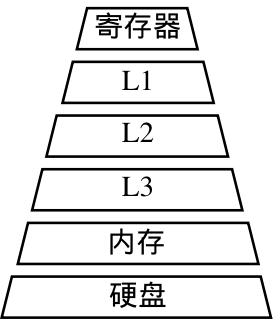
\includegraphics[scale=0.6]{figs/ch09/ch09-storage.png}
\caption{计算机分层存储架构}
\label{fig:ch09/ch09-fusion-storage}
\end{figure}

算子融合带来的性能上的收益主要来自两个方面,一是通过融合,充分利用寄存器和缓存,避免多个算子运算时,数据在CPU和内存之间的存储和读取的耗时。如图\ref{fig:ch09/ch09-fusion-storage},可以看到计算机的储存系统,从最靠近cpu的寄存器L1、L2等多级缓存,到内存、硬盘,其存储的容量越来越大,但读取数据的耗时也越来越大。融合后,前一次计算的结果可以先暂存在CPU的寄存器(Register)或者缓存(Cache)中,下一次计算直接从寄存器或者缓存中读取,减少了内存读写的IO次数。二是通过融合,可以将一些计算量提前完成,避免了前向推理时的冗余计算或者循环冗余计算。

\begin{figure}[h]
\centering
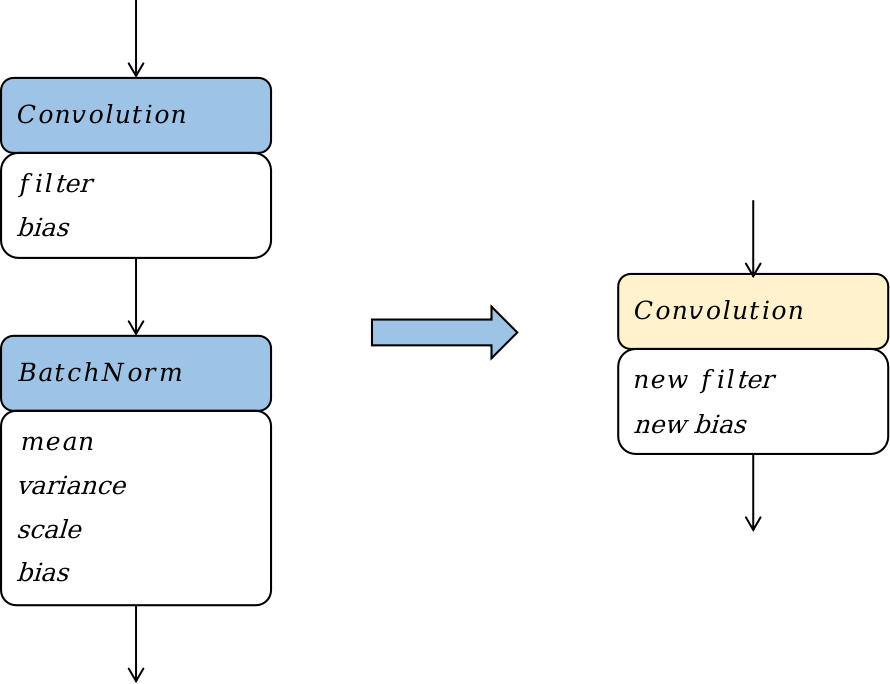
\includegraphics[scale=0.6]{figs/ch09/ch09-conv-bn-fusion.png}
\caption{Convolution + Batchnorm算子融合}
\label{fig:ch09/ch09-conv-bn-fusion}
\end{figure}

如图\ref{fig:ch09/ch09-conv-bn-fusion},我们以Convolution算子和Batchnorm算子的融合为例,阐述算子融合的基本原理,图中蓝色框表示算子,黄色框表示融合后新增或者改变的算子,白色框表示算子中的权重或者常数张量。其融合的过程是一个计算表达式简化的过程,Convolution算子的计算过程可以等效为一个矩阵乘,其公式可以表达为\ref{equ:ch09-conv-equation}。

\begin{equation}\label{equ:ch09-conv-equation}
\bm{Y_{conv}}=\bm{W_{conv}}*\bm{X_{conv}}+\bm{B_{conv}}
\end{equation}

这里我们不需要理解公式\ref{equ:ch09-conv-equation}中每个变量的含义,只需要注意到一点,该公式是$\bm{Y_{conv}}$关于$\bm{X_{conv}}$的,其他符号均表示常量。

Batchnorm算子的计算过程如公式\ref{equ:ch09-bn-equation}所示。

\begin{equation}\label{equ:ch09-bn-equation}
\bm{Y_{bn}}=\gamma\frac{\bm{X_{bn}}-\mu_{\mathcal{B}}}{\sqrt{{\sigma_{\mathcal{B}}}^{2}+\epsilon}}+\beta
\end{equation}

同样,这里我们不需要理解batchnorm中的所有参数的含义,只需要了解公式\ref{equ:ch09-bn-equation}是$\bm{Y_{bn}}$关于$\bm{X_{bn}}$的,其他符号均表示常量。

如图\ref{fig:ch09/ch09-conv-bn-fusion},当Convlution算子的输出作为Batchnorm输入时,最终Batchnorm算子的计算公式也就是要求$\bm{Y_{bn}}$关于$\bm{X_{conv}}$的计算公式,我们将$\bm{Y_{conv}}$代入到$\bm{X_{bn}}$,然后将常数项合并提取后,可以得到公式\ref{equ:ch09-conv-bn-equation-3}。

\begin{equation}\label{equ:ch09-conv-bn-equation-3}
\bm{Y_{bn}}=\bm{A}*\bm{X_{conv}}+\bm{B}
\end{equation}

其中$\bm{A}$和$\bm{B}$为两个矩阵。可以看到,公式\ref{equ:ch09-conv-bn-equation-3}其实就是一个Convolution的计算公式。这个结果表明,在模型部署时,我们可以将Convolution和Batchnorm两个算子的计算等价为一个Convolution算子。我们将上述以计算公式的合并和简化为基础的算子融合称为计算公式融合。

在Convolution算子和Batchnorm算子融合的前后,网络结构相当于减少了一个Batchnorm算子,相应的网络中的参数量和网络所需的计算量都减少了;同时由于算子数量的减少,访存次数也相应地减少了。综合来看,该融合Pattern优化了模型部署时的功耗、性能,同时对于模型的体积大小也有少许收益。
    
在融合过程中,Convolution计算公式和Batchnorm计算公式中被认为是常量的符号在训练时均为参数,并不是常量。训练阶段如果进行该融合会导致模型参数的缺失。从该融合Pattern的结果来看,融合后网络中减少了一个Batchnorm算子,减少了一个Batchnorm算子的参数量,其实就是改变了深度神经网络的算法,会影响到网络的准确率,这是不可接受的。所以Convolution算子与Batchnorm算子的融合一般是在部署阶段特有的一种优化手段,其优化效果我们以MinsSpore Lite为例,构造了包含一个Convolution和一个Batchnorm的sample网络,分别以样例网络和mobilenet-v2网络为例,在华为Mate30手机上,以两线程运行模型推理,取3000轮推理的平均时耗作为模型推理性能的指标,对比融合前后该指标的变化。从表\ref{tab:ch09/ch09-conv-bn-fusion}可以看到,对于sample网络和mobilenet-v2网络,融合后分别获得了8.5\%和11.7\%的推理性能提升,这个性能提升非常可观。并且这个性能提升没有带来任何的副作用,也没有对于硬件或算子库的提出额外要求。

\begin{table}
\centering
\caption{Convolution + Batchnorm融合前后推理性能(单位:ms)}
\label{tab:ch09/ch09-conv-bn-fusion}
\begin{tabular}{|l|c|c|}
\hline
&sample&mobilenet-v2\\
\hline
before fusion&0.035&15.415\\
after fusion&0.031&13.606\\
\hline
\end{tabular}
\end{table}

\subsection{算子替换}
算子替换,即将模型中某些算子替换计算逻辑一致但对于在线部署更友好的算子。算子替换的原理是通过合并同类项、提取公因式等数学方法,将算子的计算公式加以简化,并将简化后的计算公式映射到某类算子上。算子替换可以达到降低计算量、降低模型大小的效果。

\begin{figure}[h]
\centering
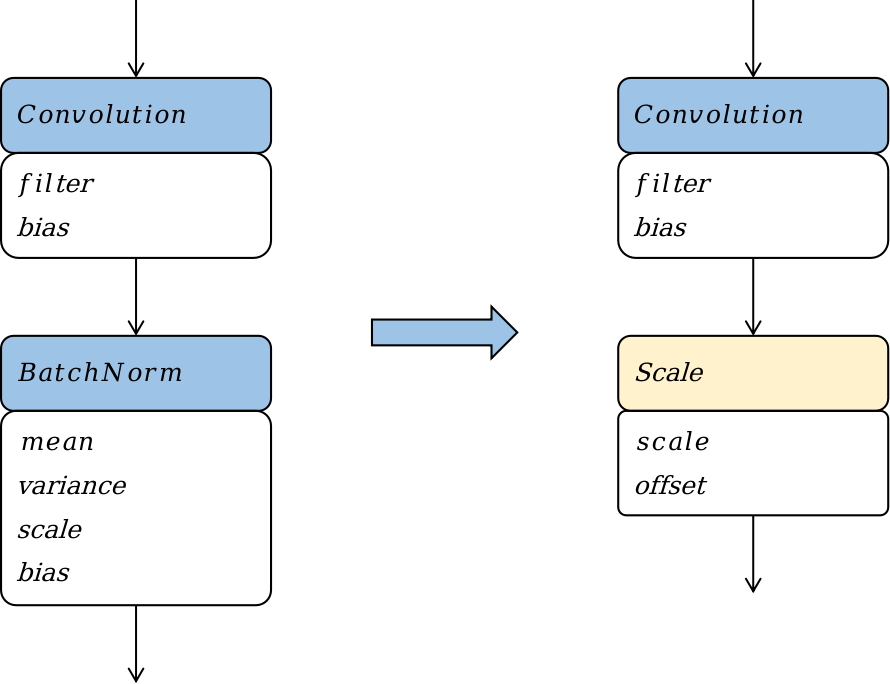
\includegraphics[scale=0.6]{figs/ch09/ch09-bn-replace.png}
\caption{Batchnorm算子替换}
\label{fig:ch09/ch09-bn-replace}
\end{figure}

如图\ref{fig:ch09/ch09-bn-replace},我们以Batchnorm算子替换成Scale算子为例,阐述算子替换的原理。我们直接将Batchnorm的计算公式\ref{equ:ch09-bn-equation}进行分解,并将常量合并简化,Batchnorm的计算公式可以写成:
\begin{equation}\label{equ:ch09-replace-scale}
\bm{Y_{bn}}=scale*\bm{X_{bn}}+offset
\end{equation}
其中scale和offset为两个标量。可以看到,计算公式简化后,我们可以将其映射到一个Scale算子。

在Batchnorm算子被替换为Scale算子的前后,网络中的参数量、计算量都减少了,该算子替换策略可以优化模型部署时的功耗和性能。同理,该算子替换优化策略只能在部署阶段才能进行,因为一方面在部署阶段Batchnorm计算公式中被认为是常量的符号,在训练时是参数并非常量。另一方面该优化策略会降低模型的参数量,改变模型的结构,降低模型的表达能力,影响训练收敛时模型的准确率。

\subsection{算子重排}
算子重排是指将模型中算子的拓扑序按照某些规则进行重新排布,在不降低模型的推理精度的前提下,降低模型推理的计算量。常用的算子重排技术有针对于Slice算子、StrideSlice算子、Crop算子等裁切类算子的前移、Reshape算子和Transpose算子的重排、BinaryOp算子的重排等。

\begin{figure}[h]
\centering
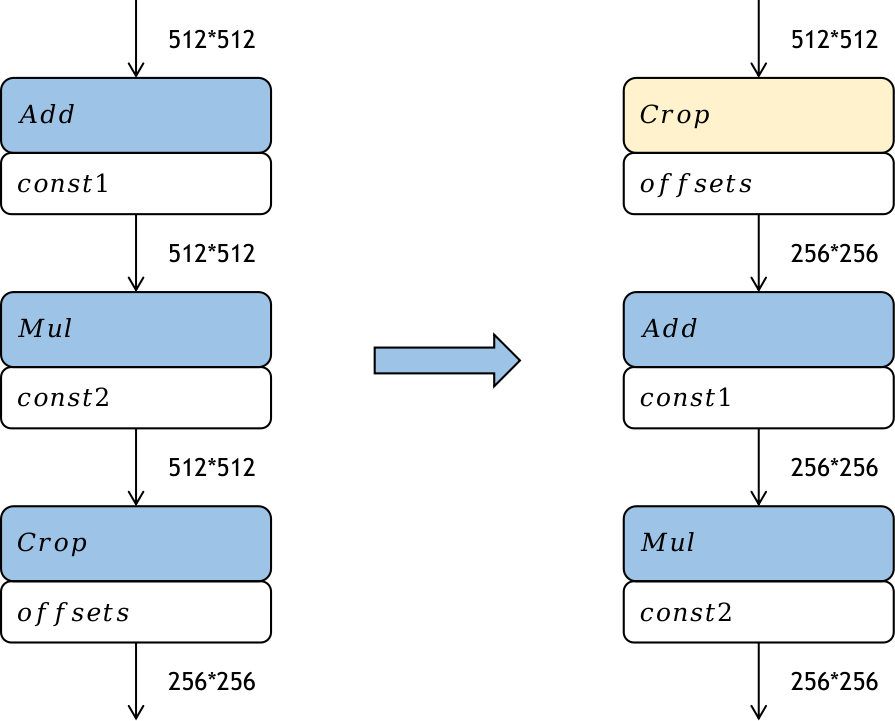
\includegraphics[scale=0.6]{figs/ch09/ch09-crop-reorder.png}
\caption{Crop算子重排}
\label{fig:ch09/ch09-crop-reorder}
\end{figure}

如图\ref{fig:ch09/ch09-crop-reorder},Crop算子是从输入的feature map中裁取一部分作为输出,经过Crop算子后,feature map的size就降低了。如果我们将这个裁切的过程前移,提前对feature map进行裁切,那么后续算子的计算量也会相应地减少,从而提高模型部署时的推理性能。Crop算子前移带来的性能提升跟Crop算子的参数有关。但是Crop算子一般只能沿着的element wise类算子前移。

通过前面的实验数据我们可以看到,通过推理前的模型优化,可以为推理的时延、功耗、内存占用带来极大的收益。


\section{模型压缩}\label{sec:ch09/ch09-model-compression}
在上一小节中,我们简要介绍了模型转换的目的,并重点讲述了模型部署时的一些常用的模型优化手段。考虑到不同场景的硬件对模型的要求不同,比如部署在手机上,对于模型的大小比较敏感,一般在兆级别。因此,对于一些较大的模型,我们往往需要通过一些模型压缩的技术,使其能满足不同计算硬件的要求。

\subsection{量化}
模型量化是指以较低的推理精度损失将连续取值(通常为FP32或者大量可能的离散值)的浮点型权重或者通过各个算子的数据定点近似(通常为INT8)为有限多个离散值的过程,如图\ref{fig:ch09/ch09-quant-minmax},T是量化前的数据范围。通过以更少的位数表示浮点数据,模型量化可以减少模型尺寸,进而减少在推理时的内存消耗,并且在一些低精度运算较快的处理器上可以增加推理速度。

\begin{figure}[h]
\centering
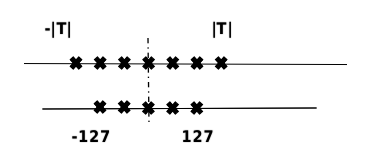
\includegraphics[scale=0.6]{figs/ch09/ch09-quant-minmax.png}
\caption{量化原理}
\label{fig:ch09/ch09-quant-minmax}
\end{figure}

计算机中不同数据类型的占用比特数及其表示的数据范围各不相同。可以根据实际业务需求将原模型量化成不同比特数的模型,一般深度神经网络的模型用单精度浮点数表示,如果能用有符号整数来近似原模型的参数,那么被量化的权重参数存储大小就可以降到原先的四分之一,用来量化的比特数越少,量化后的模型压缩率越高。工业界目前最常用的量化位数是8比特,低于8比特的量化被称为低比特量化。1比特是模型压缩的极限,可以将模型压缩为1/32,在推理时也可以使用高效的XNOR和BitCount位运算来提升推理速度。

另外,根据量化数据表示的原始数据范围是否均匀,还可以将量化方法分为线性量化和非线性量化。实际的深度神经网络的权重和激活值通常是不均匀的,因此理论上使用非线性量化能够达到更高的精度,但在实际推理中非线性量化的计算复杂度较高,通常使用线性量化。下面着重介绍线性量化的原理。

%上述公式中第一个称为量化,第二个称为反量化。     $$r=s*(q-z)$$
假设r表示量化前的浮点数,量化后的整数q可以表示为:
    \begin{equation}
        q=clip(round(\frac{r}{s}+z),q_{min},q_{max})
    \end{equation}
$round(\cdot)$和$clip(\cdot)$分别表示取整和截断操作,$q_{min}$和$q_{max}$是量化后的最小值和最大值。$s$是数据量化的间隔,$z$是表示数据偏移的偏置,$z$为0的量化被称为对称(Symmetric)量化,不为0的量化称为非对称(Asymmetric)量化。对称量化可以避免量化算子在推理中计算z相关的部分,降低推理时的计算复杂度;非对称量化可以根据实际数据的分布确定最小值和最小值,可以更加充分的利用量化数据信息,使得计算精度更高。

根据量化参数$s$和$z$的共享范围,量化方法可以分为逐层量化和逐通道量化。逐层量化以一层网络为量化单位,每层网络的一组量化参数;逐通道量化以一层网络的每个量化通道为单位,每个通道单独使用一组量化参数。逐通道量化由于量化粒度更细,能获得更高的量化精度,但计算也更复杂。

根据量化过程中是否需要训练,可以将模型量化分为量化感知训练(Quantization Aware Training, QAT)和训练后量化(Post Training Quantization, PTQ)两种,其中感知量化训练是指在模型训练过程中加入伪量化算子,通过训练时统计输入输出的数据范围可以提升量化后模型的精度,适用于对模型精度要求较高的场景;训练后量化指对训练后的模型直接量化,只需要少量校准数据,适用于追求高易用性和缺乏训练资源的场景。
    
\subsubsection{量化感知训练}

量化感知训练是在训练过程中模拟量化,利用伪量化节点将量化带来的精度变化计入训练误差,使得优化器能在训练过程中尽量减少量化误差,得到更高的模型精度。量化感知训练的具体流程如下:
 \begin{itemize}
    \item 初始化:设置权重和激活值的范围$q_{min}$和$q_{max}$的初始值;
    \item 构建模拟量化网络:在需要量化的权重和激活值后插入伪量化节点;
    \item 量化训练:重复执行以下步骤直到网络收敛,计算量化网络层的权重和激活值的范围$q_{min}$和$q_{max}$,前向计算反向传播更新网络权重参数;
    \item 导出量化网络:获取$q_{min}$和$q_{max}$,并计算量化参数$s$和$z$;
    根据公式计算权重的量化整数值,并替换对应网络层的参数和数据类型;
    删除伪量化节点,在量化网络层前后分别插入量化和反量化算子。
\end{itemize}

\subsubsection{训练后量化}

训练后量化也可以分成两种,权重量化和全量化。权重量化仅量化模型的权重以压缩模型的大小,在推理时将权重反量化为原始的FP32数据,后续推理流程与普通的FP32模型一致。权重量化的好处是不需要校准数据集,不需要实现量化算子,且模型的精度误差较小,由于实际推理使用的仍然是FP32算子,所以推理性能不会提高。全量化不仅会量化模型的权重,还会量化模型的激活值,在模型推理时执行量化算子来加快模型的推理速度、为了量化激活值,需要用户提供一定数量的校准数据集用于统计每一层激活值的分布,并对量化后的算子做校准。校准数据集可以来自训练数据集或者真实场景的输入数据,需要数量通常非常小。在做训练后量化时会以校准数据集为输入,执行推理流程然后统计每层激活值的数据分布并得到相应的量化参数,具体的操作流程如下:
 \begin{itemize}
    \item 使用直方图统计的方式得到原始FP32数据的统计分布$P_f$;
    \item 在给定的搜索空间中选取若干个$q_{min}$和$q_{max}$分别对激活值量化,得到量化后的数据$Q_q$;
    \item 使用直方图统计得到$Q_q$的统计分布;
    \item 计算每个$Q_q$与$P_f$的统计分布差异,并找到差异性最低的一个对应的$q_{min}$和$q_{max}$来计算相应的量化参数,常见的用于度量分布差异的指标包括KL散度(Kullback-Leibler Divergence)、对称KL散度(Symmetric Kullback-Leibler Divergence)和JS散度(Jenson-Shannon Divergence)。
 \end{itemize}
 
  除此之外,由于量化存在固有误差,还需要校正量化误差。以矩阵乘为例,$a=\sum_{i=1}^Nw_ix_i+b$,w表示权重,x表示激活值,b表示偏置。首先需要对量化的均值做校正,对fp32算子和量化算子输出的每个通道求平均,假设某个通道i的fp32算子输出均值为$a_i$,量化算子反量化输出均值为$a_{qi}$,将这个通道两个均值的差$a_i-a_q$加到对应的通道上即可使得最终的输出均值和fp32一致。另外还需要保证量化后的分布和量化前是一致的,设某个通道权重数据的均值、方差为$E(w_c)$、$||w_c-E(w_c)||$,量化后的均值和方差为$E(\hat{w_c})$、$||\hat{w_c}-E(\hat{w_c})||$,对权重做如下校正:
        $$\hat{w_c}\leftarrow\zeta_c(\hat{w_c}+u_c)$$
        $$u_c=E(w_c)-E(\hat{w_c})$$
        $$\zeta_c=\frac{||w_c-E(w_c)||}{||\hat{w_c}-E(\hat{w_c})||}$$

 量化方法作为一种通用的模型压缩方法,可以大幅提升神经网络存储和压缩的效率,已经取得了广泛的应用。

\subsection{模型稀疏}
模型稀疏是通过去除神经网络中部分组件(如权重、特征图、卷积核)降低网络的存储和计算代价,它和模型权重量化、权重共享、池化等方法一样,属于一种为达到降低模型计算复杂度的目标而引入的一种强归纳偏置。
\subsubsection{模型稀疏的动机}
因为卷积神经网络中的卷积计算可以被看作输入数据和卷积核中权重的加权线性组合,所以细小的权重对输出数据就具有相对较小的影响。对模型进行稀疏操作的合理性主要来源于两方面的假设:
\begin{itemize}
    \item 其一,针对权重参数来说,当前许多神经网络模型存在过参数化(Over-parameterized)的现象,动辄具有几千万甚至数亿规模的参数量。
    \item 其二,针对模型推理过程中生成的激活值特征图,对于许多检测、分类、分割等视觉任务来说激活值特征图中能利用的有效信息相对于整张图仅占较小的比例。
\end{itemize}

根据以上描述按照模型稀疏性来源的不同,主要分为权重稀疏和激活值稀疏,它们的目的都是为了减少模型当中的冗余成分来达到降低计算量和模型存储的需求。具体来说,对模型进行稀疏就是根据模型的连接强弱程度(一般根据权重或激活的绝对值大小),对一些强度较弱的连接进行剪枝(将权重参数或激活值置为0)来达到模型稀疏并提高模型推理性能的目的。特别地,我们将模型权重或激活值张量中0值所占的比例称为模型稀疏度。一般而言,模型稀疏度越高带来的模型准确率下降越大,因此我们的目标是尽可能在提高模型稀疏度的同时保证模型准确率下降较小。

实际上,如同神经网络本身的发明受到了神经生物学启发一样,神经网络模型稀疏方法同样受到了神经生物学的启发。在一些神经生物学的发现中,人类以及大多数哺乳动物的大脑都会出现一种叫做突触修剪的活动。突触修剪即神经元的轴突和树突发生衰退和完全死亡,这一活动发生在哺乳动物的婴幼儿时期,然后一直持续到成年以后。这种突触修剪机制不断简化和重构哺乳动物大脑的神经元连接,使得哺乳动物的大脑能以更低的能量获得更高效的工作方式。

\subsubsection{结构与非结构化稀疏}
首先我们考虑权重稀疏,对于权重稀疏来说,按照稀疏模式的不同,主要分为结构化和非结构化稀疏。简单来讲,结构化稀疏就是在通道或者卷积核层面对模型进行剪枝。这种稀疏方式能够得到规则且规模更小的权重矩阵,因此比较适合CPU和GPU进行加速计算。但与此同时,结构化稀疏是一种粗粒度的稀疏方式,将会对模型的推理准确率造成较大的下降。

而非结构化稀疏,可以对权重张量中任意位置的权重进行裁剪,因此这种稀疏方式属于细粒度的稀疏。这种稀疏方式相对于结构化稀疏,造成的模型准确率下降较小。但是也正是因为这种不规则的稀疏方式,导致稀疏后的模型难以利用硬件获得较高的加速比。其背后原因主要有以下几点:
\begin{itemize}
    \item 不规则排布的模型权重矩阵会带来大量的控制流指令,比如由于大量0值的存在,我们会不可避免地引入大量if-else分支判断指令,因此会降低指令层面的并行度。
    \item 权重矩阵的不规则内存排布会造成线程发散和负载不均衡,而不同卷积核往往是利用多线程进行计算的,因此这也影响了线程层面的并行度。
    \item 权重矩阵的不规则内存排布造成了较低的访存效率,因为它降低了数据的局部性以及缓存命中率。
\end{itemize}

为了解决以上非结构化稀疏带来的种种问题,近期出现的研究当中通过引入特定稀疏模式将结构化稀疏和非结构化稀疏结合了起来,从而一定程度上兼具结构化和非结构化稀疏的优点并克服了两者的缺点。

\subsubsection{稀疏策略}
明确了模型稀疏的对象之后,我们需要确定模型稀疏的具体策略,具体来说我们需要决定何时对模型进行稀疏以及如何对模型进行稀疏。目前最常见模型稀疏的一般流程为:预训练、剪枝、微调。具体而言,我们首先需要训练得到一个收敛的稠密模型,然后在此基础上进行稀疏和微调。选择在预训练之后进行稀疏动作的原因基于这样一个共识,即预训练模型的参数蕴含了学习到的知识,继承这些知识然后进行稀疏得到的模型效果要比从头开始训练好。除了基于预训练模型进行进行一步修剪之外,训练和剪枝交替进行也是一种常用的策略。相比于一步修剪的方法,这种逐步的修剪方式,使得训练和剪枝紧密结合,可以更有效地发现冗余的卷积核,被广泛采用于现代神经网络剪枝方法中。

以下通过一个具体实例(Deep Compression~(\cite{han2015deep})) 来说明如何进行网络修剪:如图\ref{fig:ch09/ch09-deepcomp}所示,在去掉大部分的权值之后,深度卷积神经网络的精度将会低于其原始的精度。对剪枝后稀疏的神经网络进行微调,可以进一步提升压缩后网络的精度。剪枝后的模型可以进一步进行量化,使用更低比特的数据来表示权值;此外,结合霍夫曼(Huffman)编码可以进一步地降低深度神经网络的存储。

\begin{figure}[h]
\centering
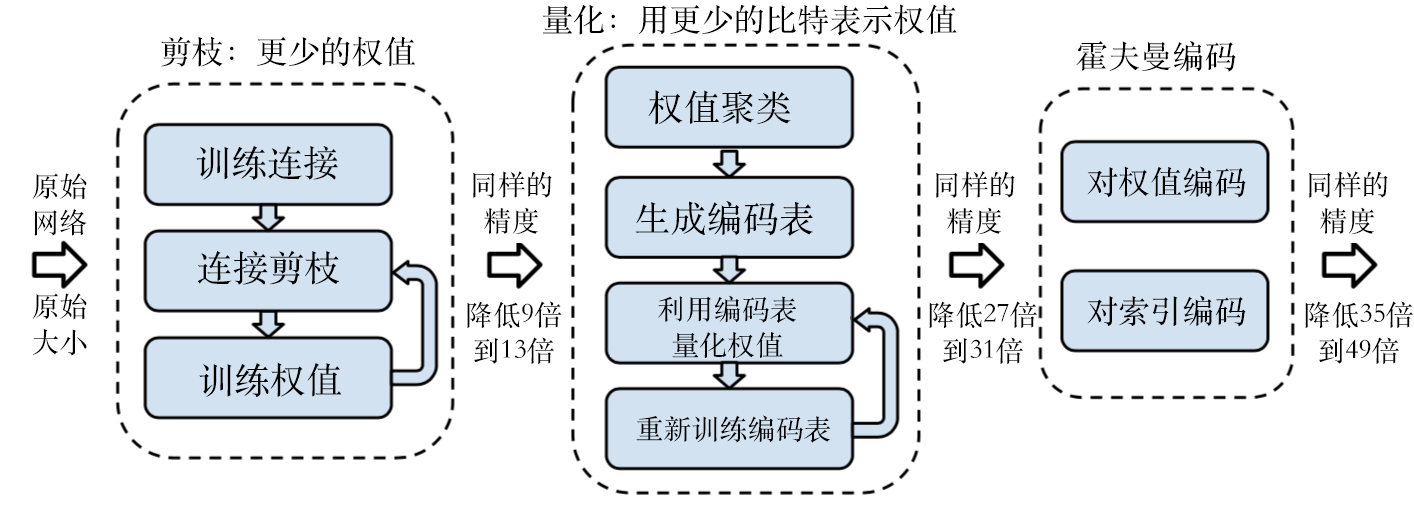
\includegraphics[scale=0.6]{figs/ch09/ch09-deepcomp.png}
\caption{Deep Compression~(\cite{han2015deep}) 算法的流程图}
\label{fig:ch09/ch09-deepcomp}
\end{figure}

除了直接去除冗余的神经元之外,基于字典学习的方法也可以用来去掉深度卷积神经网络中无用的权值~(\cite{bagherinezhad2017lcnn})。通过学习一系列卷积核的基,可以把原始卷积核变换到系数域上并且它们稀疏。比如,Bagherinezhad 等人~(\cite{bagherinezhad2017lcnn}) 将原始卷积核分解成卷积核的基和稀疏系数的加权线性组合。

\subsection{知识蒸馏}
知识蒸馏,也被称为教师-学生神经网络学习算法,已经受到业界越来越多的关注。大型深度模型在实践中往往会获得良好的性能,因为当考虑新数据时,过度参数化会提高泛化性能。在知识蒸馏中,小模型(学生模型)通常是由一个大模型(教师模型)监督,算法的关键问题是如何从老师模型转换的知识传授给学生模型。通过把一个全新的更深的更窄结构的深度神经网络当作学生神经网络,然后把一个预先训练好的神经网络模型当作教师神经网络。利用这个教师神经网络模型来帮助学生神经网络模型的算法是当下的一个研究热点。

Hinton等人~(\cite{Distill})首先提出了教师神经网络-学生神经网络学习框架,通过最小化两个神经网络之间的差异来学习一个更窄更深的神经网络。记教师神经网络为$\mathcal{N}_{T}$,它的参数为$\theta_T$,同时记学生神经网络为$\mathcal{N}_{S}$,相应的参数为$\theta_S$。一般而言,学生神经网络相较于教师神经网络具有更少的参数。

% 记这两个神经网络模型在softmax分类器中输入的数据为$z_T$和$z_S$,相应的输出数据为:
% \begin{equation}
% o_S = \frac{e^{\theta_S^{\top}z_S}}{||e^{\theta_S^{\top}z_S}||_1}, \quad o_T = \frac{e^{\theta_T^{\top}z_T}}{||e^{\theta_T^{\top}z_T}||_1},
% \end{equation}

文献~(\cite{Distill})提出的知识蒸馏(knowledge distillation,KD)方法,同时令学生神经网络的分类结果接近真实标签并且令学生神经网络的分类结果接近于教师神经网络的分类结果,即,
\begin{equation}
\mathcal{L}_{KD}(\theta_S) = \mathcal{H}(o_S,\mathbf{y}) +\lambda\mathcal{H}(\tau(o_S),\tau(o_T)),
\label{c2Fcn:distill}
\end{equation}
其中,$\mathcal{H}(\cdot,\cdot)$是交叉熵函数,$o_S$和$o_T$分别是学生网络和教师网络的输出,$\mathbf{y}$是标签。公式~\ref{c2Fcn:distill}中的第一项使得学生神经网络的分类结果接近预期的真实标签,而第二项的目的是提取教师神经网络中的有用信息并传递给学生神经网络,$\lambda$是一个权值参数用来平衡两个目标函数。$\tau(\cdot)$是一个软化(soften)函数,将网络输出变得更加平滑。

% 且将$\tau>1$,输入数据变换为:
% \begin{equation}
% \tau(o_S) = \frac{e^{\theta_S^{\top}z_S}/\tau}{||e^{\theta_S^{\top}z_S}/\tau||_1}, \quad \tau(o_T) = \frac{e^{\theta_T^{\top}z_T}/\tau}{||e^{\theta_T^{\top}z_T}/\tau||_1}.
% \end{equation}

公式~\ref{c2Fcn:distill}仅仅从教师神经网络分类器输出的数据中提取有价值的信息,并没有从其它中间层去将教师神经网络的信息进行挖掘。因此,Romero等人~(\cite{FitNet})进一步地开发了一种学习轻型学生神经网络的方法,该算法可以从教师神经网络中任意的一层来传递有用的信息给学生神经网络。此外,事实上,并不是所有的输入数据对卷积神经网络的计算和完成后续的任务都是有用的。例如,在一张包含一个动物的图像中,对分类和识别结果比较重要的是动物所在的区域,而不是那些无用的背景信息。所以,有选择性地从教师神经网络的特征图中提取信息是一个更高效的方式。于是,Zagoruyko和Komodakis~(\cite{attentionTS})提出了一种基于感知(attention)损失函数的学习方法来提升学生神经网络的性能,如图~\ref{c2Fig:AttentionTS}所示。该算法在学习学生神经网络的过程中,引入了Attention模块,选择性地将教师神经网络中的信息传递给学生神经网络,并帮助其进行训练。

\begin{figure}[t]
\begin{center}
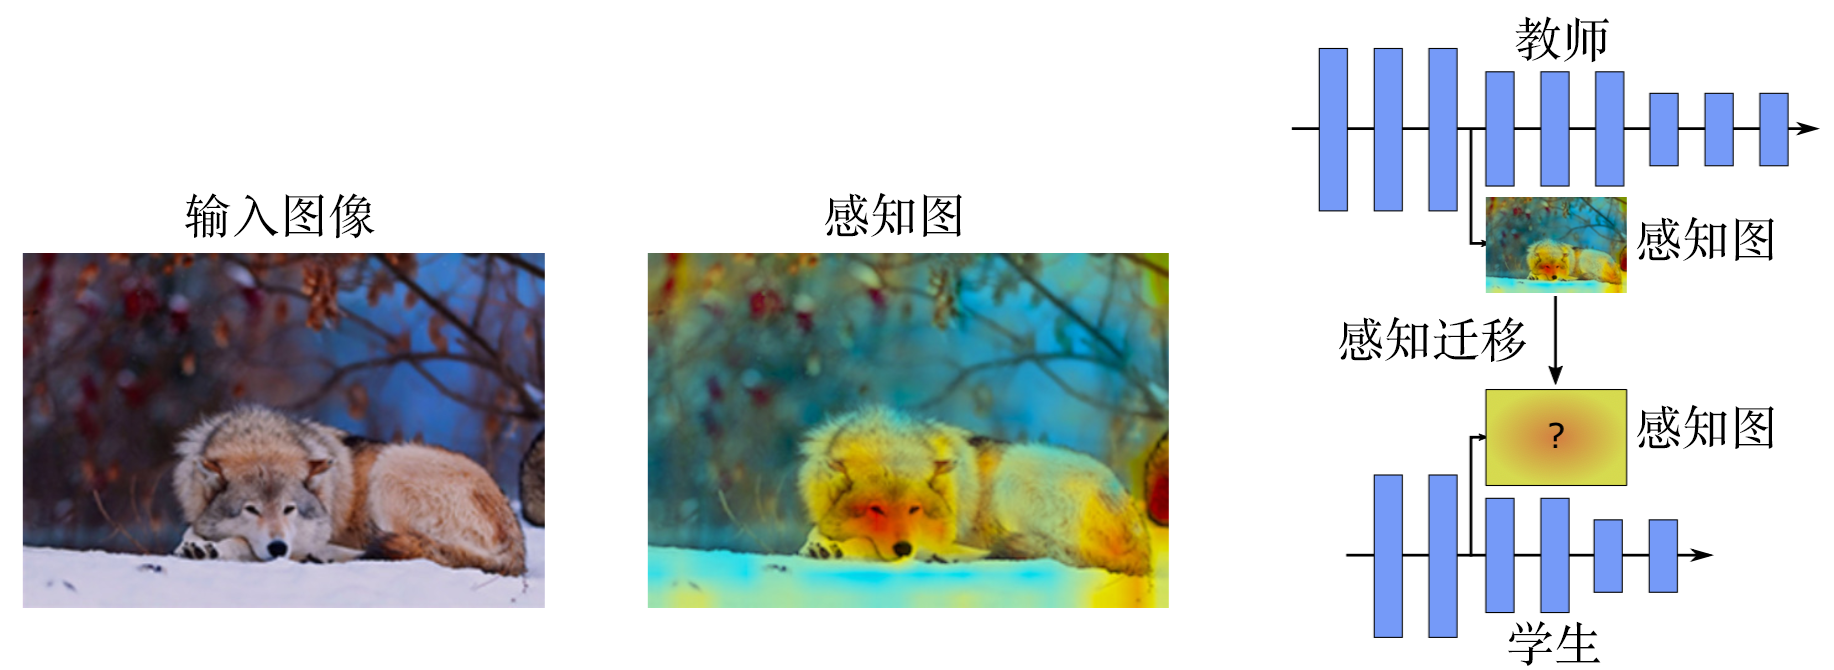
\includegraphics[width=0.95\linewidth]{figs/ch09/ch09-AttentionTS.png}
\caption{文献~(\cite{attentionTS})所提出的教师神经网络-学生神经网络学习算法,该算法在学习学生神经网络的过程中,引入了感知模块(Attention),选择性地将教师神经网络中的信息传递给学生神经网络,并帮助其进行训练。感知图可以识别输入图像不同位置对最终分类结果的重要性,并从教师网络传递到学生网络。}
\label{c2Fig:AttentionTS}
\end{center}
\end{figure}

知识蒸馏是一种有效的帮助小网络优化的方法,能够进一步和剪枝、量化等其他压缩方法结合,训练得到精度高、计算量小的高效模型。

\section{模型推理}
训练模型经过前面的转换、压缩等流程后,需要部署在计算硬件上进行推理。执行推理主要包含以下步骤:

1. 前处理:将原始数据处理成适合网络输入的数据。

2. 执行推理:将离线转换得到的模型部署到设备上执行推理流程,根据输入数据计算得到输出数据。

3. 后处理:模型的输出结果做进一步的加工处理,如筛选阈值。


\subsection{前处理与后处理}
\subsubsection{前处理}
前处理主要完成数据预处理,在现实问题中,我们得到的原始数据往往非常混乱,机器学习模型无法识别并从中提取信息。数据预处理的目的是将原始数据例如图片、语音、文本等,处理成适合网络输入的tensor数据,并消除其中无关的信息,恢复有用的真实信息,增强有关信息的可检测性,最大限度地简化数据,从而改进模型的特征抽取、图像分割、匹配和识别等可靠性。

常见的数据预处理手段有:

1. 特征编码:将描述特征的原始数据编码成数字,输入给机器学习模型,因为它们只能处理数字数据。常见的编码方法有:离散化、序号编码、One-hot编码,二进制编码等;

2. 数据归一化:修改数据的值使其达到共同的标度但不改变它们之间的相关性,消除数据指标之间的量纲影响。常用的技术有:Min-Max归一化将数据缩放到给定范围,Z-score归一化使数据符合正态分布;

3. 处理离群值: 离群值是与数据中的其他值保持一定距离的数据点,适当地排除离群值可以提升模型的准确性。

针对特定的原始数据,往往存在特定的数据处理手段。在前述8.2“机器学习数据基本类型及常见数据变换方式”章节中,分别详细介绍了图像、音频、文本等数据的预处理方法。
\subsubsection{后处理}
通常,模型推理结束后,需要把推理的输出数据传递给用户完成后处理,常见的数据后处理手段有:

1. 连续数据离散化:模型实际用于预测离散数据,例如商品数量时,用回归模型预测得到的是连续值,需要四取五入、取上下限阈值等得到实际结果;

2. 数据可视化:将数据图形化、表格化,便于找到数据之间的关系,来决定下一步的分析策略;

3. 手动拉宽预测范围:回归模型往往预测不出很大或很小的值,结果都集中在中部区域。例如医院的化验数据,通常是要根据异常值诊断疾病。手动拉宽预测范围,将偏离正常范围的值乘一个系数,可以放大两侧的数据,得到更准确的预测结果。

\subsection{并行计算}\label{sec:ch09/ch09-parallel-inference}

为提升推理的性能,需要重复利用多核的能力,所以一般推理框架会引入多线程机制。主要的思路是将算子的输入数据进行切分,通过多线程去执行不同数据切片,实现算子并行计算,从而成倍提升算子计算性能。
 
 \begin{figure}[h]
\centering
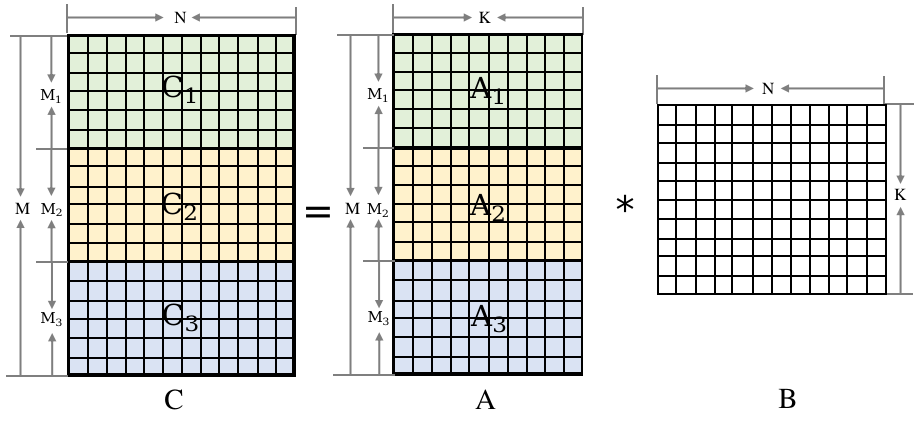
\includegraphics[scale=0.8]{figs/ch09/ch09-parallel.png}
\caption{矩阵乘数据切分}
\label{figs:ch09_parallel}
\end{figure}

如图所示,对于矩阵乘可以按左矩阵的行进行切分,可以利用三个线程分别计算A1*B,A2*B,A3*B,实现矩阵乘多线程并行计算。

为方便算子并行计算,同时避免频繁创建销毁线程的开销,推理框架一般会使用线程池机制。业界有两种较为通用的做法:

1. 使用OpenMp编程接口:OpenMP(Open Multi-Processing)是一套支持跨平台共享内存方式的多线程并发的编程API,如算子并行最常用的接口"parallel for",实现for循环体的代码被多线程并行执行。

2. 推理框架实现针对算子并行计算的线程池,相对OpenMp提供的接口会更有针对性,性能会更高,且更轻量。

\subsection{算子优化}\label{sec:ch09/ch09-kernel-optimization}
在部署AI模型时,我们期望模型执行训练或推理的时间尽可能地短,以获得更优越的性能。对于一个固定的深度学习网络,框架调度的时间占比往往很小,性能的瓶颈就在算子的执行。下面从硬件指令和算法角度介绍一些算子优化的方法。

\subsubsection{硬件指令优化}
绝大多数的设备上都有CPU,因此算子在CPU上的时间尤为重要,下面介绍一下在ARM CPU硬件指令优化的方法。

1. 汇编语言

开发者使用的C++、Java等高级编程语言会通过编译器输出为机器指令码序列,而高级编程语言能做的事通常受编译器所限,汇编语言是靠近机器的语言,可以一对一实现任何指令码序列,编写的程序存储空间占用少、执行速度快、效率优于高级编程语言。

在实际应用中,最好是程序的大部分用高级语言编写,运行性能要求很高的部分用汇编语言来编写,通过混合编程实现优势互补。深度学习的卷积、矩阵乘等算子涉及大量的计算,使用汇编语言能够给模型训练和推理性能带来数十到数百倍量级的提升。

下面以ARMv8系列处理器为例,介绍和硬件指令相关的优化。

2. 寄存器与NEON指令

ARMv8系列的CPU上有32个NEON寄存器v0-v31,如图\ref{fig:ch09/ch09-register}所示,NEON寄存器v0可存放128bit的数据,即4个float32,8个float16,16个int8等。

\begin{figure}[h]
\centering
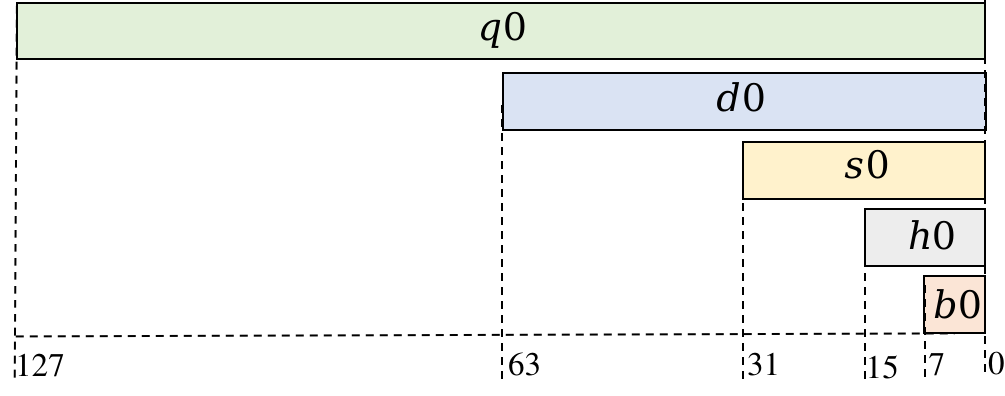
\includegraphics[scale=0.5]{figs/ch09/ch09-register.png}
\caption{ARMv8处理器NEON寄存器v0的结构}
\label{fig:ch09/ch09-register}
\end{figure}

针对该处理器,可以采用SIMD(Single Instruction,Multiple Data,单指令、多数据)提升数据存取计算的速度。相比于单数据操作指令,NEON指令可以一次性操作NEON寄存器的多个数据。例如:对于浮点数的fmla指令,用法为fmla v0.4s, v1.4s, v2.4s,如图\ref{fig:ch09/ch09-fmla}所示,用于将v1和v2两个寄存器中相对应的float值相乘累加到v0的值上。

\begin{figure}[h]
\centering
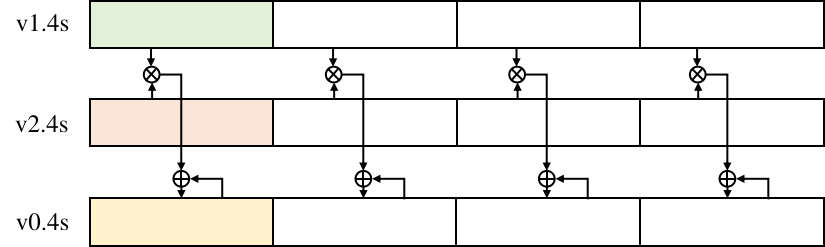
\includegraphics[scale=0.5]{figs/ch09/ch09-fmla.png}
\caption{fmla指令计算功能}
\label{fig:ch09/ch09-fmla}
\end{figure}

3. 汇编语言优化

对于已知功能的汇编语言程序来说,计算类指令通常是固定的,性能的瓶颈就在非计算指令上。如图\ref{fig:ch09/ch09-fusion-storage}所示,计算机各存储设备类似于一个金字塔结构,最顶层空间最小,但是速度最快,最底层速度最慢,但是空间最大。L1-L3统称为cache(高速缓冲存储器),CPU访问数据时,会首先访问位于CPU内部的cache,没找到再访问CPU之外的主存,此时引入了缓存命中率的概念来描述在cache中完成数据存取的占比。要想提升程序的性能,缓存命中率要尽可能的高。

下面简单列举一些提升缓存命中率、优化汇编性能的手段:

(1)循环展开:尽可能使用更多的寄存器,以代码体积换性能;

(2)指令重排:打乱不同执行单元的指令以提高流水线的利用率,提前有延迟的指令以减轻延迟,减少指令前后的数据依赖等;

(3)寄存器分块:合理分块NEON寄存器,减少寄存器空闲,增加寄存器复用;

(4)计算数据重排:尽量保证读写指令内存连续,提高缓存命中率;

(5)使用预取指令:将要使用到的数据从主存提前载入缓存,减少访问延迟。
\subsubsection{算法优化}

多数AI模型的推理时间主要耗费在卷积、矩阵乘算子的计算上,占到了整网百分之九十甚至更多的时间。本小节主要介绍卷积算子算法方面的优化手段,可以应用到各种硬件设备上。
卷积的计算可以转换为两个矩阵相乘,在前述5.3.3小节中,已经详细介绍了矩阵乘GEMM运算的优化。对于不同的硬件,确定合适的矩阵分块,优化数据访存与指令并行,可以最大限度的发挥硬件的算力,提升推理性能。

1.Img2col

将卷积的计算转换为矩阵乘,一般采用Img2col的方法实现。在常见的神经网络中,卷积的输入通常都是4维的,默认采用的数据排布方式为NHWC,如图\ref{fig:ch09/ch09-conv_nhwc}所示,是一个卷积示意图。输入维度为(1,IH,IW,IC),卷积核维度为(OC,KH,KW,IC),输出维度为(1,OH,OW,OC)。

\begin{figure}[h]
\centering
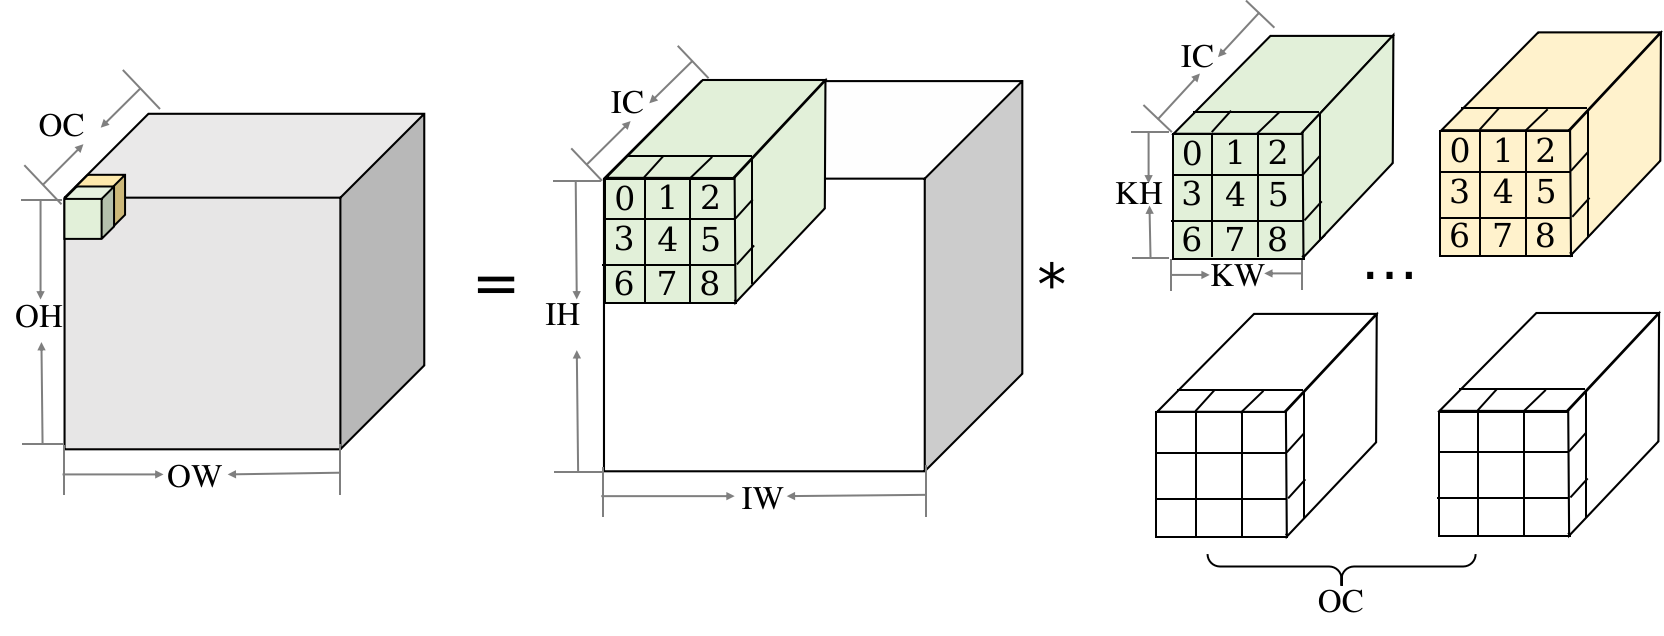
\includegraphics[scale=0.5]{figs/ch09/ch09-conv_nhwc.png}
\caption{通用卷积示意图}
\label{fig:ch09/ch09-conv_nhwc}
\end{figure}

对卷积的Img2col规则如下。如图\ref{fig:ch09/ch09-img2col_input}所示,对该输入做重排,得到的矩阵见右侧,行数对应输出的OH*OW的个数;每个行向量里,先排列计算一个输出点所需要输入上第一个通道的KH*KW个数据,再按次序排列之后的通道,直到通道IC。

\begin{figure}[h]
\centering
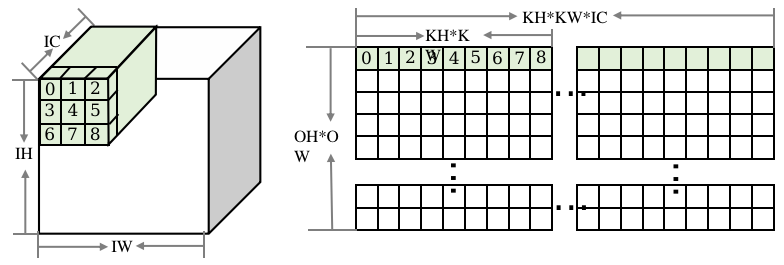
\includegraphics[scale=0.85]{figs/ch09/ch09-img2col_input.png}
\caption{输入Img2col的矩阵}
\label{fig:ch09/ch09-img2col_input}
\end{figure}

如图\ref{fig:ch09/ch09-img2col_weight}所示,对权重数据做重排。将1个卷积核展开为权重矩阵的一列,因此共有OC列,每个列向量上先排列第一个输入通道上KH*KW的数据,再依次排列后面的通道直到IC。通过重排,卷积的计算就可以转换为两个矩阵相乘的求解。在实际实现时,Img2col和GEMM的数据重排会同时进行,以节省运行时间。

\begin{figure}[h]
\centering
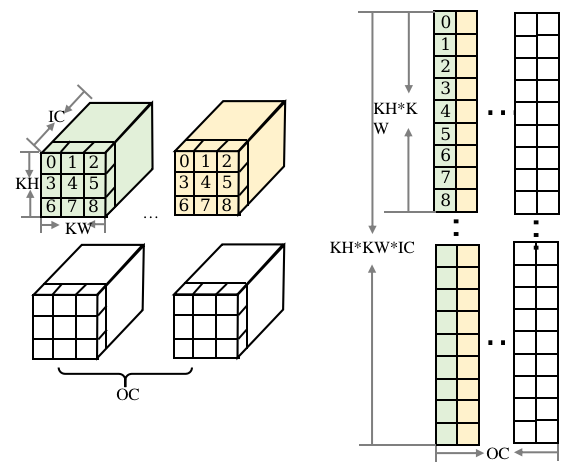
\includegraphics[scale=0.85]{figs/ch09/ch09-img2col_weight.png}
\caption{卷积核Img2col的矩阵}
\label{fig:ch09/ch09-img2col_weight}
\end{figure}

2.Winograd算法

卷积计算归根到底是矩阵乘法,两个二维矩阵相乘的时间复杂度是$O(n^3)$。我们可以使用Winograd来降低矩阵乘法的复杂度。

以一维卷积运算为例,记为F(m,r),其中,m代表输出的个数,r为卷积核的个数。输入为$d=[d_0 \ d_0 \ d_2 \ d_3]$,卷积核为$g=[g_0 \ g_0 \ g_2]^T$,该卷积计算可以写成矩阵形式如公式\ref{equ:ch09-conv-matmul-one-dimension}所示,需要6次乘法和4次加法。

\begin{equation}\label{equ:ch09-conv-matmul-one-dimension}
F(2, 3)=
\left[ \begin{matrix} d_0 & d_0 & d_2 \\ d_1 & d_2 & d_3 \end{matrix} \right] \left[ \begin{matrix} g_0 \\ g_1 \\ g_2 \end{matrix} \right]=
\left[ \begin{matrix} y_0 \\ y_1 \end{matrix} \right]
\end{equation}

可以观察到,卷积运算转换为矩阵乘法时输入矩阵中存在着重复元素$d_1$和$d_2$,因此,卷积转换的矩阵乘法相对一般的矩阵乘有了优化空间。可以通过计算中间变量$m_0-m_3$得到矩阵乘的结果,见公式\ref{equ:ch09-conv-2-winograd}:

\begin{equation}\label{equ:ch09-conv-2-winograd}
F(2, 3)=
\left[ \begin{matrix} d_0 & d_0 & d_2 \\ d_1 & d_2 & d_3 \end{matrix} \right] \left[ \begin{matrix} g_0 \\ g_1 \\ g_2 \end{matrix} \right]=
\left[ \begin{matrix} m_0+m_1+m_2 \\ m_1-m_2+m_3 \end{matrix} \right]
\end{equation}

其中,$m_0-m_3$的分别见公式\ref{equ:ch09-winograd-param}:

\begin{equation}\label{equ:ch09-winograd-param}
\begin{aligned}
m_0=(d_0-d_2)*g_0 \\
m_1=(d_1+d_2)*(\frac{g_0+g_1+g_2}{2}) \\
m_2=(d_0-d_2)*(\frac{g_0-g_1+g_2}{2}) \\
m_2=(d_1-d_3)*g_2
\end{aligned}
\end{equation}

通过$m_0-m_3$间接计算r1,r2,需要的运算次数包括:输入d的4次加法;输出m的4次乘法和4次加法。在推理阶段,权重的数值是常量,因此卷积核上的运算可以在图编译阶段计算,不计入在线的run时间。所以总的运算次数为4次乘法和8次加法,与直接运算的6次乘法和4次加法相比,乘法次数减少,加法次数增加。在计算机中,乘法一般比加法慢,通过减少乘法次数,增加少量加法,可以实现加速。

计算过程写成矩阵形式如公式\ref{equ:ch09-winograd-matrix}所示,其中,⊙为对应位置相乘,A、B、G都是常量矩阵。这里写成矩阵计算是为了表达清晰,实际使用时,按照公式\ref{equ:ch09-winograd-param}手写展开的计算速度更快。

\begin{equation}\label{equ:ch09-winograd-matrix}
\mathbf{Y}=\mathbf{A^T}(\mathbf{G}g)*(\mathbf{B^T}d)
\end{equation}

\begin{equation}\label{equ:ch09-winograd-matrix-bt}
\mathbf{B^T}=
\left[ \begin{matrix} 1 & 0 & -1 & 0 \\ 0 & 1 & 1 & 0 \\ 0 & -1 & 1 & 0 \\ 0 & 1 & 0 & -1 \end{matrix} \right]
\end{equation}

\begin{equation}\label{equ:ch09-winograd-matrix-g}
\mathbf{G}=
\left[ \begin{matrix} 1 & 0 & 0 \\ 0.5 & 0.5 & 0.5 \\ 0.5 & -0.5 & 0.5 \\ 0 & 0 & 1 \end{matrix} \right]
\end{equation}

\begin{equation}\label{equ:ch09-winograd-matrix-at}
\mathbf{A^T}=
\left[ \begin{matrix} 1 & 1 & -1 & 0 \\ 0 & 1 & -1 & -1  \end{matrix} \right] \\
\end{equation}

通常深度学习领域通常使用的都是2D卷积,将F(2,3)扩展到F(2x2,3x3),可以写成矩阵形式,如公式\ref{equ:ch09-winograd-two-dimension-matrix}所示。此时,Winograd算法的乘法次数为16,而直接卷积的乘法次数为36,降低了2.25倍的乘法计算复杂度。

\begin{equation}\label{equ:ch09-winograd-two-dimension-matrix}
\mathbf{Y}=\mathbf{A^T}(\mathbf{G}g\mathbf{G^T})*(\mathbf{B^T}d\mathbf{B})\mathbf{A}
\end{equation}

Winograd算法的整个计算过程在逻辑上可以分为4步,如图\ref{fig:ch09/ch09-winograd}所示:

\begin{figure}[h]
\centering
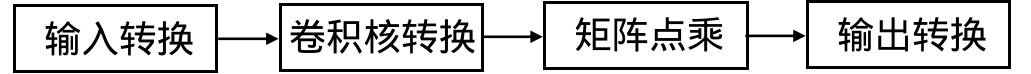
\includegraphics[scale=0.5]{figs/ch09/ch09-winograd.png}
\caption{winograd步骤示意图}
\label{fig:ch09/ch09-winograd}
\end{figure}

针对任意的输出大小,要使用F(2x2,3x3)的Winograd算法,需要将输出切分成2x2的块,找到对应的输入,按照上述的四个步骤,就可以求出对应的输出值。当然,Winograd算法并不局限于求解F(2x2,3x3),针对任意的F(m*m,r*r),都可以找到适当的常量矩阵A、B、G,通过间接计算的方式减少乘法次数。但是随着m、r的增大,输入、输出涉及的加法以及常量权重的乘法次数都在增加,那么乘法次数带来的计算量下降会被加法和常量乘法所抵消。因此,在实际使用场景中,还需要根据Winograd的实际收益来选择。

本小节主要介绍了模型推理时的数据处理和性能优化手段。选择合适的数据处理方法,可以更好地提取输入特征,处理输出结果。并行计算以及算子级别的硬件指令与算法优化可以最大限度的发挥硬件的算力。除此之后,内存的占用及访问速率也是影响推理性能的重要因素,因此推理时需要设计合理的内存复用策略,关于内存复用的策略我们在编译器后端章节已经做了阐述。


\section{模型的安全保护}\label{sec:ch09/ch09-distributed-inference}
xxx。

\subsection{概述}
xxx。


\subsection{模型混淆}
xxx。

\subsection{xxx}
。

\section{模型部署实践}
\subsection{图像检测在安卓手机上的部署实践}

\section{总结}
\begin{itemize}
    \item 不同的模型部署场景下,通常对于模型大小、运行时内存占用、推理时延和推理功耗等指标有限制。
    \item 针对模型大小指标,通常在离线阶段通过模型压缩技术来优化,比如量化技术、剪枝技术、知识蒸馏技术等,除此之外,一部分模型优化技术,比如融合技术(\ref{sec:ch09/ch09-kernel-fusion})等,也有助于模型轻量化,不过其效果比较微弱。
    \item 总结未完。
\end{itemize}
\bibliographystyle{spbasic}
\bibliography{references}
